%!TEX TS-program = pdflatex
%!TEX root = progetto_finale.tex
%!TEX encoding = UTF-8 Unicode

\chapter{Validazione}

Check if requirements from Chapter 2 have been fullfilled. Quantitative tests (simulations) and screenshots of the interfaces are put here.

\section{Compilazione ed esecuzione del codice}

Istruzioni per la compilazione ed esecuzione
Scompattare il contenuto della cartella in una posizione a scelta. 
Avviare erlang e posizionarsi all'interno della root del progetto. 
Se assente, creare la cartella ``ebin'' sempre nella root.
Eseguire il comando
\lstinline|make:all().|
Spostarsi nella cartella "ebin" tramite il comando
\lstinline|cd("ebin").|
Avviare l'environment tramite il comando
\lstinline| PID_ENV = main:start_project().|
Viene avviato l'environment 


\section{Test eseguiti}

\section{Controllo requisiti}

\chapter{Implementazione}

Il linguaggio scelto per l'implementazione del progetto è Erlang. Esso è stato selezionato per diversi motivi tra cui: fornisce nativamente il supporto alla gestione di messaggi e scambio di essi tra diverse entità; permette di creare in poche righe di codice diversi beam a cui poter richiedere dei servizi; fornisce librerie tramite le quali è possibile creare facilmente gli automi e le interazioni fra essi. Inoltre supporta nativamente la programmazione concorrente semplificando la gestione da parte dello sviluppatore della programmazione parallela. Infine essendo un linguaggio funzionale, che quindi non presenta memoria condivisa, non permette l'esistenza della race condition tra processi.

In questo progetto non utilizzate piattaforme esterne di alcun genere poiché si assume che l'autenticazione tra utente e applicazione per il servizio sia già stata effettuata.

Essendo un'architettura peer to peer, non è necessaria alcuna piattaforma a parte l'autenticazione cliente - servizio.

\section{Generazione dell'ambiente virtuale}
Il problema della modellazione di una città è stato risolto con un grafo pesato connesso non orientato: si assume che se due nodi sono connessi è perché vi è una strada tra di essi ed è bidirezionale. Il peso indica quanto costa attraversarla. 

\subsection{Entità presenti}
Si immagina che i diversi nodi siano posizionati all'interno di un piano cartesiano, pertanto possiedono delle coordinate che ne indicano la posizione. Questo permette di capire la distanza tra di essi e quindi se diverse entità riescono a comunicare tra di loro.

\subsection{Componenti del grafo} \label{componenti_grafo_citta}
Ogni nodo del grafo possiede quattro proprietà:
\begin{itemize}
	\item attributo nome: generato del tipo ``aa'', ``ab'', ``ac'', ... incrementale per ogni nodo.
	\item attributo id: numero incrementale per ogni nodo a partire da 0. Utilizzato per la definizione del grafo della città.
	\item Coordinate X e Y: definiscono la posizione del nodo all'interno del piano cartesiano rappresentante la città.
\end{itemize}

Per quanto riguarda gli archi, essi posseggono tre proprietà:
\begin{itemize}
	\item ID\_Nodo\_1 - ID\_Nodo\_2: indica quali nodi collega.
	\item Peso: indica il peso dell'arco, calcolato in funzione della distanza tra i nodi che collega l'arco.
\end{itemize}

Infine vengono selezionati alcuni nodi tra quelli del grafo che conterranno le colonnine di ricarica. Per far questo è stato applicato il seguente algoritmo:
\begin{enumerate}
	\item In base al numero totale delle colonnine, il piano cartesiano viene suddiviso in parti uguali.
	\item Selezione di un nodo casuale all'interno della parte creata a cui assegnare la colonnina.
\end{enumerate}

\subsection{Parametri per la generazione}
Il linguaggio utilizzato per la generazione della città è python. All'interno del file ``map\_generator'' è possibile impostare i diversi parametri per la generazione della città, vale a dire:
\begin{itemize}
	\item WEIGHT\_MIN: Peso minimo degli archi.
	\item WEIGHT\_MAX:  Peso massimo degli archi.
	\item TOTAL\_NODES: Totale numero di nodi del grafo.
	\item TOTAL\_EDGES:  Totale numero di archi del grafo.
	\item TOTAL\_CHARGING\_COLS:  Totale numero delle colonnine di ricarica nel grafo.
	\item CARTESIAN\_SIDE:  Lato del quadrato cartesiano utilizzato per la mappa.
\end{itemize}

Per quanto riguarda il numero di colonnine, esso non è garantito essere rispettato per il seguente motivo: come spiegato precedentemente, l'algoritmo utilizzato suddivide il piano in parti uguali ma potrebbe capitare nel caso esse siano piccole che non vi sia alcun nodo all'interno. Dato che in ogni zona è presente al più una colonnina, può capitare che non siano presenti zone con nodi liberi a cui assegnare le rimanenti.

\subsection{File generati}
Lo script in python crea cinque file:
\begin{itemize}
	\item ``map.pdf'': I dati generati per il grafo vengono esportati nel formato dot e da esso viene generato questo file al cui interno è presente una rappresentazione visuale del grafo: sono presenti i nodi con le proprietà descritte precedentemente e gli archi con delle etichette rappresentanti il loro peso. Un esempio del pdf prodotto è l'immagine \ref{fig:esempio_citta_dot}.
	\item ``map.png'': Rappresentazione visuale delle posizioni dei nodi all'interno del piano cartesiano. I nodi colorati di rosso sono quelli contenenti le colonnine di ricarica. Un esempio del png prodotto è l'immagine \ref{fig:esempio_citta_png}.
	\item ``city\_map\_nodes.dat'': file testuale contenente i dati dei nodi formattati in modo da essere compatibili con la struttura creata in erlang. Un esempio è il seguente:
	\begin{lstlisting}
		10
		a 0 1 4
		b 1 2 12
		c 2 3 12
		d 3 3 16
		e 4 5 2
		...
	\end{lstlisting}
	\item ``city\_map\_graph.dat'': file testuale contenente i dati del grafo formattato in modo da essere compatibile con la libreria utilizzata in erlang. Un esempio è il seguente:
	\begin{lstlisting}
		10 30 undirected d
		6 0 17
		0 1 12
		1 8 18
		8 4 20
		4 7 14
		7 3 21
		3 9 18
		...
	\end{lstlisting}
	\item ``city\_map\_charging\_cols.dat'': file testuale contenente i dati dei nodi delle colonnine. Essi sono formattati in modo da essere compatibili con la struttura creata in erlang. Lo stile è il medesimo del file ``city\_map\_nodes.dat''.
	
\end{itemize}

\begin{figure}[htbp]
	\centering
	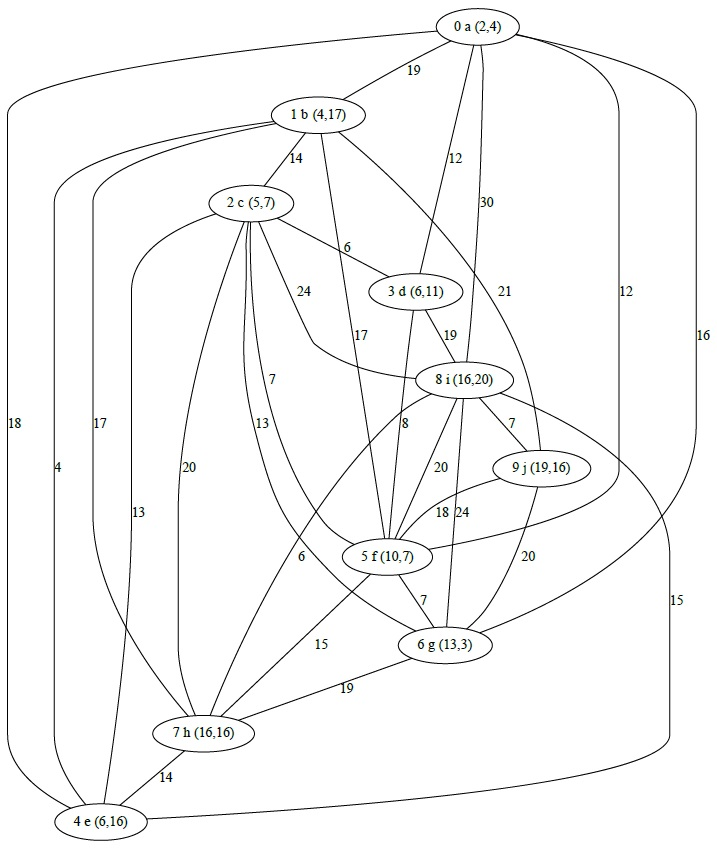
\includegraphics[width=14cm]{esempio_citta_dot.jpg}
	\caption{Esempio di grafo utilizzato per la simulazione della città.}
	\label{fig:esempio_citta_dot}
\end{figure}


\begin{figure}[htbp]
	\centering
	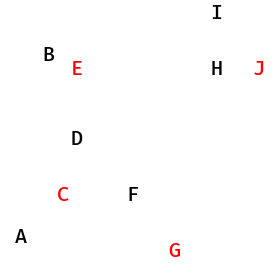
\includegraphics[width=8cm]{esempio_citta_png.jpg}
	\caption{Esempio del posizionamento dei nodi all'interno della città.}
	\label{fig:esempio_citta_png}
\end{figure}

\section{Entità Ambiente}

\section{Mappa città e relativi algoritmi}
Il record ``city'' contiene cinque parametri:
\begin{itemize}
	\item city\_graph: grafo caricato dalla libreria descritta al punto \ref{libreria_algoritmi}.
	\item total\_nodes: numero totale dei nodi del grafo.
	\item total\_edges: numero totale di archi del grafo.
	\item nodes: nodi presenti nella mappa secondo la struttura definita al punto \ref{nodi_citta}.
	\item column\_positions: sottoinsieme dei nodi che contengono le colonine.
\end{itemize}

Esso contiene lo stato attuale della città dal punto di vista topologico. Le sue componenti vengono utilizzate da diverse entità del sistema per diversi scopi:
L'automa elezione inserire riferimento ne utilizza il city\_graph per calcolare i costi della macchina.

L'entità ambiente inserire riferimento ne utlizza i nodi per generare casualmente le posizion iniziali di macchine e utenti.

Il Gps Server inserire riferimento ne utilizza i nodi per creare la propria struttura dove tiene traccia della posizione attuale delle entità presenti in un determinato istante nella città


\subsection{Nodi città}\label{nodi_citta}
Come già descritto al punto \ref{componenti_grafo_citta}, ogni nodo possiede diverse proprietà che vengono memorizzate nell'apposito record definito in questo modo:
\begin{itemize}
	\item name: nome del nodo
	\item id: identificativo numerico del nodo, utlizzato per la sua codifica nel grafo. Questo è necessario poichè la libreria descritta al punto \ref{libreria_algoritmi} per identificare i nodi utilizza il loro id numerico.
	\item pos\_x: coordinata sull'asse delle ascisse del nodo.
	\item pos\_y: coordinata sull'asse delle ordinate del nodo.
\end{itemize}

All'avvio l'entità ambiente, tramite il modulo ``node\_utils'', carica la lista dei nodi presenti nel file ``city\_map\_nodes.dat'' e la lista presente nel file ``city\_map\_charging\_cols.dat''. Queste due liste vengono utilizzate per identificare quali sono i nodi della città e quali di essi sono colonnine. 

La scelta di separarle è stata effettuata poichè nella ricerca della colonnina più vicina alla posizione della macchina è sufficiente calcolare la distanza tra ogni colonnina e il punto desiderato, senza scorrere tutti i nodi della mappa.

Il metodo ``get\_nearest\_col/3'' presente nel modulo ``city\_map'' permette di sapere quale colonnina sia quella più geograficamente vicina al nodo passato come parametro.

Il modulo ``node\_utils'' fornisce i diversi getter per ottenere le informazioni desiderate a partire dalla lista e un identificativo per un determinato nodo. Esso inoltre fornisce dei metodi per ottenere un nodo random presente, con la possibilità di escludere un nodo. Questa proprietà viene utilizzata nella generazione delle richieste degli utentei come spiegato al punto REF\_CREATING\_REQUEST.

\subsection{Libreria per algoritmi} \label{libreria_algoritmi}
Data la natura del progetto, è necessario poter gestire grafi ed applicare ad essi l'algoritmo di Dijkstra per il calcolo dei cammini minimi tra due nodi di esso. Per eseguire questo compito, si è scelto di utilizzare la libreria ``erlang-algorithms'' fornita da Aggelos Giantsios, reperibile al sito \url{https://github.com/aggelgian/erlang-algorithms}. Essa fornisce sia le strutture base che gli algoritmi da applicare ad esse.

Di questa libreria vengono principalmente tre funzionalità:
\begin{itemize}
	\item graph:from\_file/1: permette, leggendo un file, di crearne il grafo associato in un'apposita struttura erlang.
	\item dijkstra:run/2: esegue l'algoritmo di dijkstra applicato al grafo passato come parametro iniziando dal nodo indicato.
	\item graph\_utils:getDataPath/2: vengono passati i risultati calcolati da dijkstra e il nodo target di cui si vuole sapere il percorso calcolato.
\end{itemize}

L'algoritmo di Dijkstra viene utilizzato nell'automa dell'elezione come spiegato al punto REF\_elezione\_automa.

\section{Moduli Gps e Server Gps}
Il problema in esame concerne la posizione delle diverse entità all'interno di una città, pertanto è necessario esse possiedano un modulo in grado di dir loro la posizione e distanza delle altre entità presenti. Per far questo è stato deciso di creare due moduli:
\begin{itemize}
	\item gps\_server: tiene traccia delle posizioni di tutte le entità.
	\item gps\_module: comunica con il server per sapere quali sono le entità vicine a lui.
\end{itemize}

\subsection{Gps Server}\label{gps_server}
Con lo scopo di simulare la ricezione dei vicini delle diverse entità, esso fornisce dei messaggi tramite i quali è possibile ottenere queste informazioni. Questo modulo utlizza quattro record:

\begin{itemize}
	\item nodeDistance: è una tupla formata da due valori, vale a dire ``dist'', che indica la distanza dal nodo che fa la richiesta, e ``entities'', che è una lista di pid. Il significato di essa è ``a questa distanza ci sono queste entità''.
	\item entity: è una tupla formata da tre valori: ``pid'', ossia il pid dell'entità, ``type'', l'atomo che contiene l'informazione sul tipo di entità, ed infine ``position'', che contiene il nome del nodo dov'è attualmente situata l'entità.
	\item nodeEntities: contiene due campi, vale a dire ``nodeData'', che contiene i dati del nodo che si sta considerando (dati come definiti al punto \ref{nodi_citta}), e ``entities'', che è una lista di pid. 
	\item gpsServerState: contiene due liste, una di entity come appena definite e una di nodeEntities.
\end{itemize}

Le funzionalità che offre il server sono principalmente due:

\begin{itemize}
	\item getNearEntities/2: i parametri che riceve sono la posizione di partenza e la potenza del segnale. Ciò che il server fa è il calcolo della distanza di tutti i nodi della mappa dal nodo di partenza e filtra questi in base al valore della potenza del segnale. Non importa l'ordine, l'output è una lista contenente i nodi entro il range che il segnale copre.
	\item getSortedEntities/2: i parametri che riceve sono la posizione di partenza e la potenza del segnale. Il server, dopo aver calcolato la distanza di tutti i nodi e filtrati in base alla distanza massima, li ordina tramite un algoritmo di sorting. L'output è una lista di pid ordinati in base alla distanza dal nodo di partenza ma senza l'informazione della distanza. Sta al richiedente estrarre il pid voluto.
\end{itemize}

In entrambi i casi vengono effettuati i seguenti passaggi: nel calcolo delle distanze, viene creata un'istanza del record ``nodeDistance'' contenente, come già spiegato, distanza e pid presenti nel nodo; poichè i pid delle entità sono presenti in liste diverse, viene applicata la funzione ``packNodes'' che estrae dal record ``nodeDistance'' i pid e ne crea una lista.

\subsection{Gps Module}\label{gps_module}
Rappresenta il modulo ``localizzatore vicini'' descritto nella parte \ref{modules}. Esso fornisce all'automa della macchina e dell'applicazione dell'utente le funzioni per il recupero delle entità vicine.



\section{Automi macchina}

\section{Entità presenti}

\section{Fornitori di servizi}

\section{Automa Elezione}

\section{Interazione tra i diversi moduli}

